\chapter{الاختبارات والنتائج}
\section{مقدمة}
في هذا الفصل سنتحدث عن مجموعة معطيات التدريب والاختبار وهي
\textLR{GOT-10k}،
وعن معايير التقييم والمقارنة الخاصة بهذه المجموعة، ومن ثم سنعرض نتائج تدريب كتلة الانتباه المضافة الخاصة بدمج السمات، ونعرض نتائج الاختبار على مجموعتي الـ
\textLR{validation,testing}.
ونعرض المقارنة بين الخوارزمية الأساسية 
\textLR{SwinTrack-Tiny}
وبين نموذجنا من حيث الأداء والسرعة والحجم.
\section{مجموعة معطيات التدريب 
	\textLR{\cite{got10k}GOT-10k}
}
اخترنا تدريب النموذج على مجموعة معطيات التدريب 
\textLR{GOT-10k}
الخاصة بعملية الملاحقة.
وهي اختصار لـ
\textLR{Generic Object Tracking GOT}،
تتكون من أكثر من 
$10000$
فيديو، لذلك سميت بـ
\textLR{GOT-10k}.
وتحوي أكثر من 
$105$
مليون مستطيل محيط محدد بشكل يدوي، بحجم ملف أكثر من 
$60GB$.
\newline
هذه الفيديوهات مقسمة إلى 
$563$
صنف من الأغراض، وإلى 
$87$
صنف من أنماط الحركة. وذلك بهدف تغطية أكبر قدر ممكن من تحديات الملاحقة الواقعية.
يوضح الشكل 
\ref{fig:got10k}
بعض من عينات مجموعة المعطيات 
\textLR{GOT-10k}.
\newline
أما الشكل 
\ref{fig:got10k-classes}
فيعبر عن عدد أصناف الأغراض في مجموعات التدريب الخاصة بالملاحقة، نلاحظ أن مجموعة المعطيات
\textLR{GOT-10k}
هي المعطيات الأكثر تنوعا ($563$ غرض)، يليها مجموعة معطيات 
\textLR{LaSOT\cite{Lasot}}
($70$ غرض).
\newline
توفر مجموعة المعطيات $5$ ملفات مع كل فيديو
\begin{itemize}
\item \textLR{groundtruth.txt}:
تحتوي على إحداثيات الزاوية العليا اليمينية من المستطيل المحيط، بالإضافة إلى أبعاد المستطيل.
\item \textLR{absence.label}:
القيمة $0$ تعبر عن وجود الغرض في الصورة، القيمة $1$ تعبر عن عدم وجود الغرض.
\item \textLR{cover.label}:
نسبة ظهور الهدف في الصورة،
$Value_{cover} \in \{0,1,2,...,8\}$
حيث تعبر القيمة $0$ عن غياب الغرض تماماً، وتعبر القيمة $8$ عن ظهور الهدف بشكل كامل.
\item \textLR{cut$\_$by$\_$image.label}:
حيث تعبر القيمة
$1$ عن وجود جزء من الغرض خارج نطاق الصورة، و تعبر القيمة $0$ عن وجود  كامل الغرض داخل نطاق الصورة.  
\item \textLR{meta$\_$info.ini}:
يحوي هذا الملف على رابط الفيديو، طوله، تردده، صنف الغرض، صنف الحركة، دقة الصورة.
\end{itemize}

\begin{figure}[H]
	\centerline{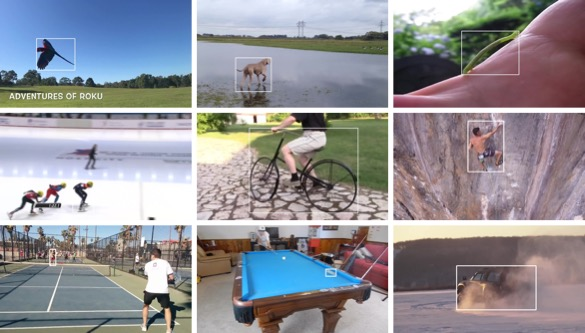
\includegraphics[width=\textwidth]{images/got10k}}
	\caption{
		\textRL{عينات من مجموعة المعطيات}
		\textLR{GOT-10k}
		\textLR{\cite{got10k}}}
	\label{fig:got10k}
\end{figure}
\begin{figure}[H]
	\centerline{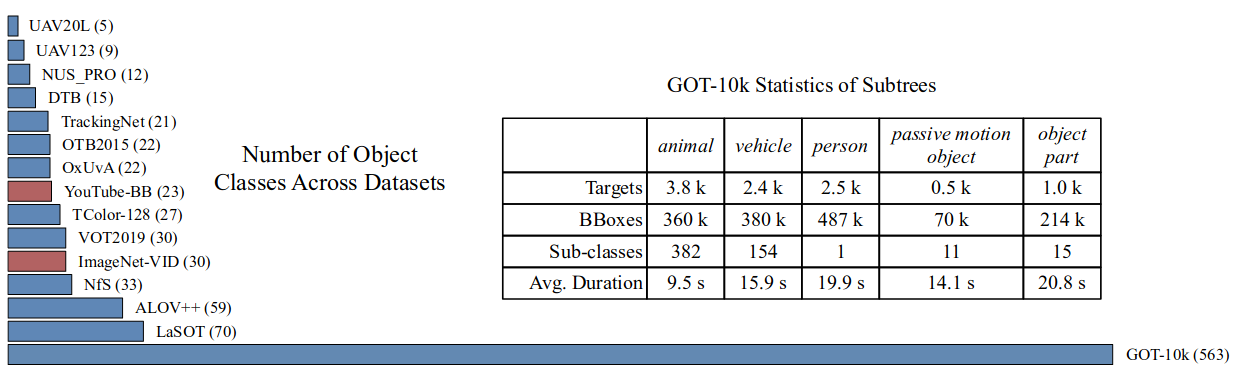
\includegraphics[width=\textwidth]{images/got10k_classes}}
	\caption{
		\textRL{عدد أصناف الأغراض في مجموعات المعطيات الخاصة بالملاحقة}
		\textLR{\cite{got10k}}}
	\label{fig:got10k-classes}
\end{figure}

هذا التصنيف لمجموعة المعطيات يفيد في تطوير خوارزميات الملاحقة، وفي إيجاد نقاط الضعف، كتحديد الحالات التي لا يستطيع فيها النموذج ملاحقة الغرض.
\subsection{معطيات الاختبار
\label{section:got10k}}
تستخدم مجموعة المعطيات
\textLR{GOT-10k}
بروتوكول
\textLR{one-shot}،
أي أنه لا يوجد تقاطع بين معطيات التدريب ومعطيات الاختبار من حيث صنف الغرض، باستثناء غرض $"$الشخص$"$.
\newline
يوضح الشكل 
\ref{fig:got10k_split}
عدد الأصناف وعدد الفيديوهات في كل مجموعة، حيث تحتوي مجموعة الاختبار على $420$ فيديو، تتألف من $84$ صنف من الأغراض، و$31$ صنف حركة.
\begin{figure}[!h]
	\centerline{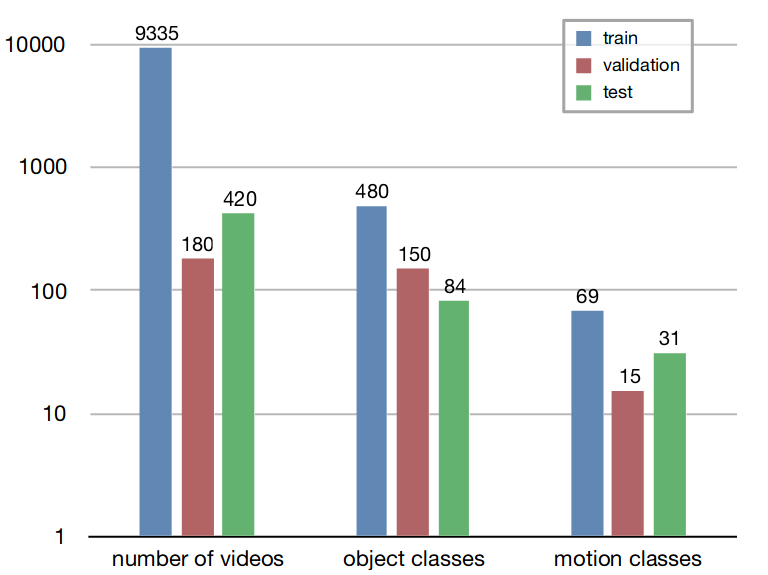
\includegraphics[scale=0.4]{images/got10k_split}}
	\caption{
		\textRL{عدد أصناف الأغراض والحركة في كل جزء من مجموعة  }
		\textLR{GOT-10k}
		\textLR{\cite{got10k}}}
	\label{fig:got10k_split}
\end{figure}
\newline
إن مجموعة الاختبار غير مزودة بالقيم الحقيقية للمستطيل المحيط، وذلك لتجنب معايرة أوزان النموذج من أجل هذه المعطيات.
لاختبار نموذج الملاحقة، نولد ملف بإحداثيات المستطيل المحيط بالهدف، هذه الاحداثيات مقدرة من قبل النموذج، ونرسله إلى مخدم خاص بمجموعة المعطيات
\textLR{GOT-10k}،
 كما يوضح الشكل
\ref{fig:got10k_submit}،
	
\begin{figure}[H]
	\centerline{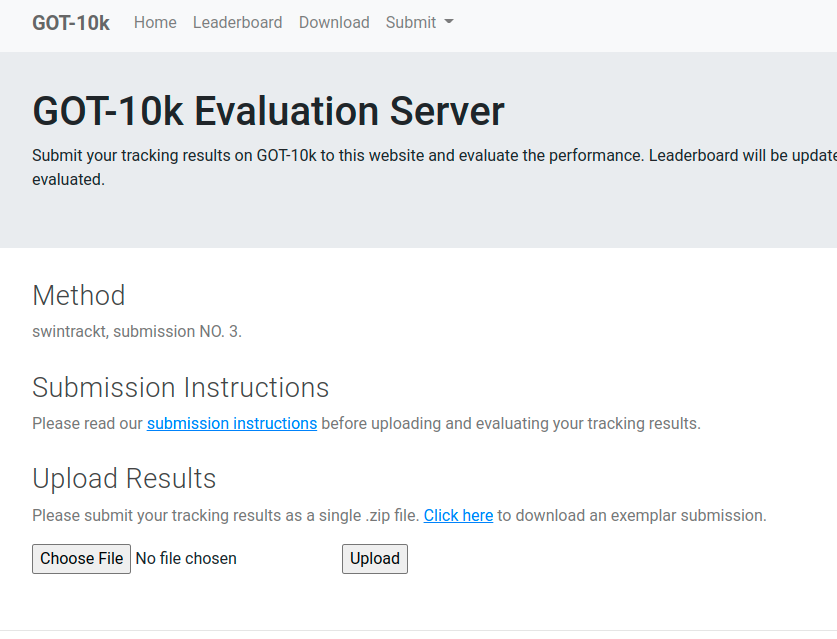
\includegraphics[width=\textwidth]{images/got10k_submit}}
	\caption{\textRL{
					\textRL{المخدم الخاص بعملية اختبار الملاحق من أجل مجموعة المعطيات}
	}}
	\label{fig:got10k_submit}
\end{figure}
\vspace{-8.0mm}
\centerline{\textRL{
				\textLR{GOT-10k}
		\textLR{\cite{got10k}}
}}	

%\begin{figure}[!h]
%	\centerline{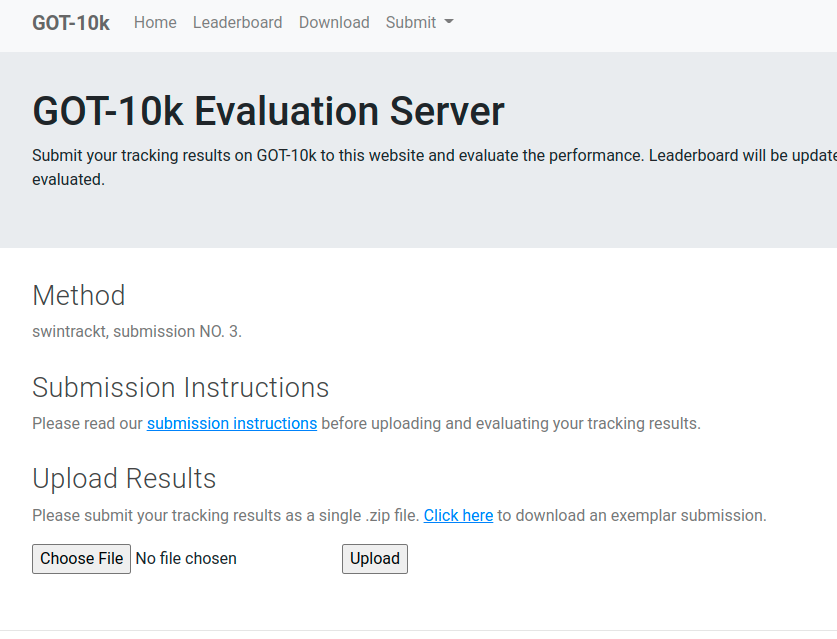
\includegraphics[width=\textwidth]{images/got10k_submit}}
%	\caption{
%		\begin{footnotesize}
%		\textRL{المخدم الخاص بعملية اختبار الملاحق من أجل مجموعة المعطيات}
%		\textLR{GOT-10k}
%		\textLR{\cite{got10k}}
%		\end{footnotesize}
%	}
%	\label{fig:got10k_submit}
%\end{figure}
حيث يمتلك هذا المخدم القيم الحقيقية ويقارنها بالقيم المرسلة، ومن ثم يحسب كل من المعياريين
$mAO,mSR$
كما في الشكل
\ref{fig:got10k_result_mai}.
\newline
لمنع استخدام المخدم للتدريب أو لتعديل أوزان النموذج بحسب نتائج الأداء، فإنه لا يسمح بإرسال أكثر من ملف خلال $48$ ساعة.
\begin{figure}[H]
	\centerline{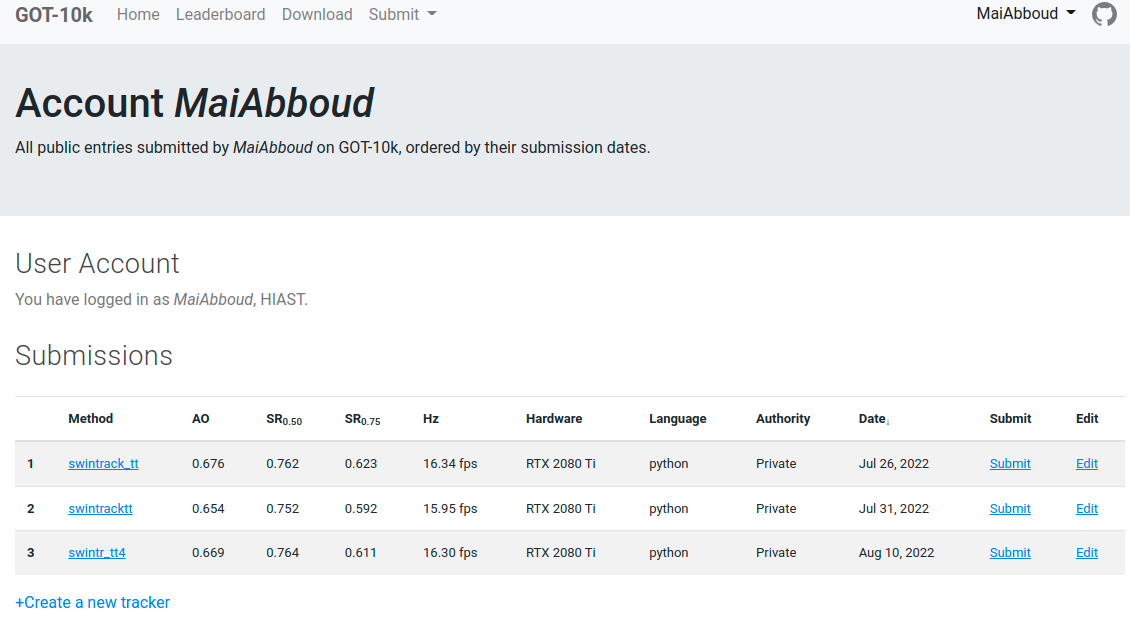
\includegraphics[width=\textwidth]{images/got10k_result_mai}}
	\caption{\textRL{
	\textRL{مثال عن نتائج اختبار بعض خوارزميات الملاحقة من أجل مجموعة المعطيات}
	}}
	\label{fig:got10k_result_mai}
\end{figure}
\vspace{-8.0mm}
\centerline{\textRL{
	\textLR{GOT-10k}
}}	

%\begin{figure}[H]
%	\centerline{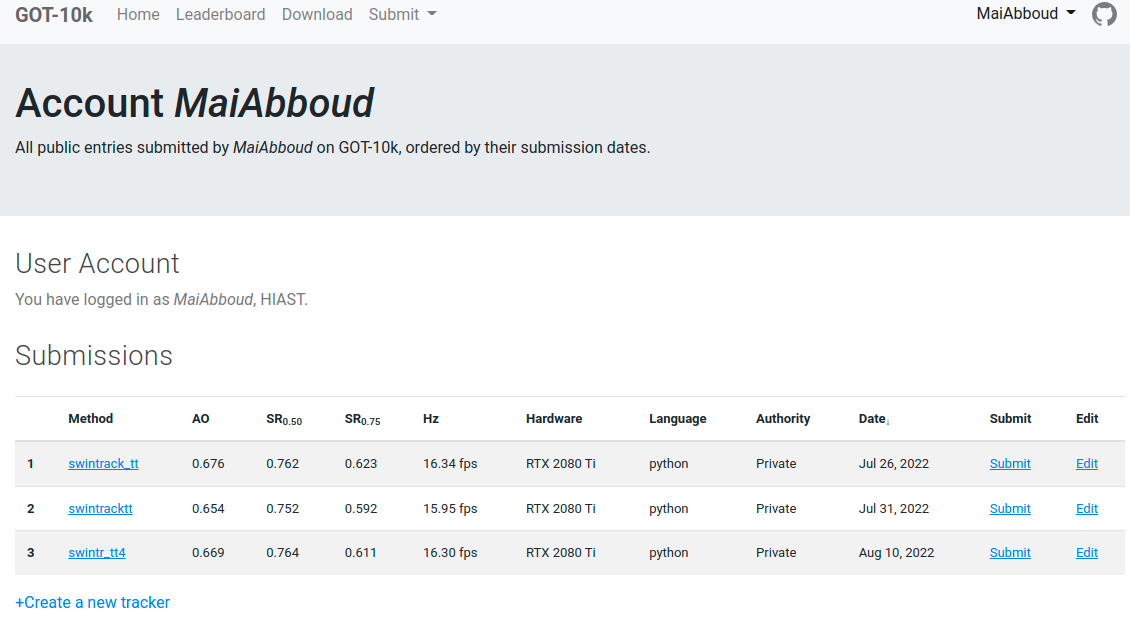
\includegraphics[width=\textwidth]{images/got10k_result_mai}}
%	\caption{
%		\begin{footnotesize}
%		\textRL{مثال عن نتائج اختبار بعض خوارزميات الملاحقة من أجل مجموعة المعطيات}
%		\textLR{GOT-10k}
%		\end{footnotesize}
%	}
%	\label{fig:got10k_result_mai}
%\end{figure}
\subsection{معايير التقييم
\textLR{Benchmarks}
\label{section:benchmark}
}
لمقارنة الملاحقات ببعضها لابد من وجود معايير لتقييم الأداء، هذه المعايير تختلف بين مجموعات المعطيات، لذلك سنذكر فقط المعايير الخاصة بمجموعة 
\textLR{GOT-10k}.
\subsubsection{المعيار الأول
\textLR{Average Overlape AO}}
يمكن تعريف 
\textLR{AO}
بأنها نسبة التقاطع إلى الاجتماع
\textLR{Intersection Over Union IOU}،
كما في الشكل
\ref{fig:iou}، 
فهي نسبة تقاطع المستطيل المحيط الحقيقي مع المستطيل المحيط المقدر من قبل الملاحق إلى إجتماع هذين المستطيلين.
\newline
\begin{figure}[H]
	\centerline{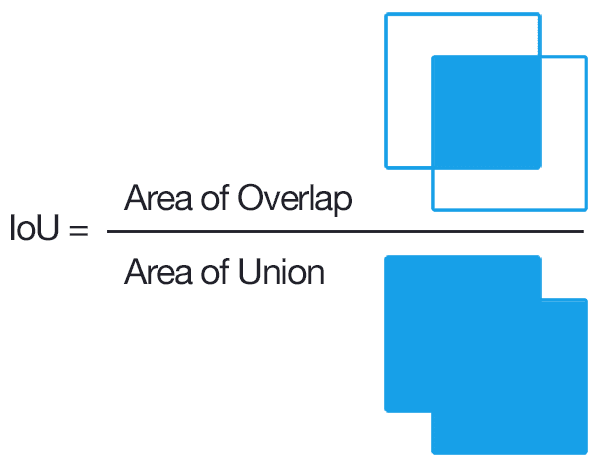
\includegraphics[scale=0.25]{images/iou_equation}}
	\caption{
		\textRL{شكل توضيحي عن }
		\textLR{IOU}
		\textLR{\cite{web:IOU_fig}}}
	\label{fig:iou}
\end{figure}
بعد الانتهاء من التدريب، ومن أجل كل 
\textLR{epoch}،
يتم اختبار النموذج بدايةً على مجموعة الـ 
\textLR{validation}.
ويتم حساب 
\textLR{mAO}،
وهي متوسط 
\textLR{AO}
من أجل كل صنف وذلك بحسب المعادلة
\begin{equation}
mAO = \frac{1}{C} \Sigma_{c=1}^C(\frac{1}{|S_c|} \Sigma_{i \in S_c}AO_i)
\end{equation}
حيث $c$ رقم الصف، $C$ عدد الصفوف، $S_c$ مجموعة الفيديوهات التي تنتمي إلى الصف $c$،
 $|S_c|$
عدد عناصر المجموعة.
\subsubsection{المعيار الثاني - معدل النجاح
\textLR{Success Rate $SR_{ratio}$}}
تقيس هذه القيمة نسبة الإطارات التي تم ملاحقتها وكان الـ
$AO$
لها
أكبر من نسبة معينة.
في معظم الأحيان يتم اظهار النتائج من أجل النسبتين 
$0.75،0.5$.
وكما في 
\textLR{AO}
فإنه يتم حساب 
$mSR_{0.75},mSR_{0.5}$
من أجل مجموعة الـ
\textLR{validation}.
\subsubsection{منحنيات التقييم - منحني النجاح 
\textLR{Success Curve}}
تعبر كل نقطة من هذه المنحني عن نسبة النجاح من أجل نسبة معينة
$threshold$،
أي التي يتجاوز فيها 
\textLR{AO}
نسبة معينة
\textLR{overlap threshold}،
كما يوضح الشكل
\ref{fig:got10k_SuccessCurve}
من أجل مجموعة من خوارزميات الملاحقة،
\begin{figure}[!h]
	\centerline{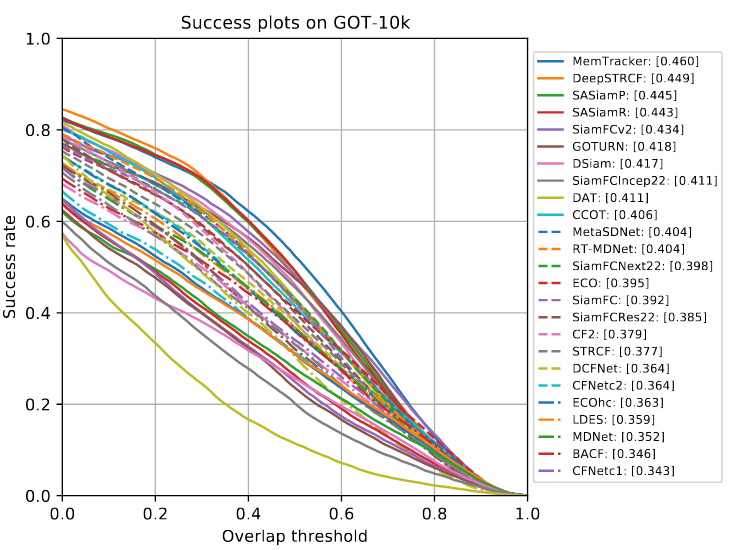
\includegraphics[width=\textwidth]{images/got10k_SuccessCurve}}
	\caption{
		\textRL{منحني النجاج من أجل عدة خوارزميات ملاحقة}
		\textLR{\cite{got10k}}}
	\label{fig:got10k_SuccessCurve}
\end{figure}
يعبر هذا المنحني من أجل القيم الصغيرة للـ
\textLR{overlap threshold}
عن الصلادة، أي عن نسبة الإطارات التي تم ملاحقتها، ومن أجل القيم الكبيرة للـ
\textLR{overlap threshold}
عن الدقة في الملاحقة.
\subsubsection{منحنيات التقييم - منحني الدقة 
	\textLR{Precision Curve}}
يعبر منحني الدقة في كل نقطة منه عن نسبة الإطارات التي بعد مركز الغرض المقدّر عن القيمة الحقيقة أقل من حد معين.
\section{النتائج}
في هذه الفقرة سنعرض نتائج النموذج الأساسي 
\textLR{SwinTrack-Tiny}،
ونتائج التجارب التي قمنا بها.
\subsection{النموذج الأساسي
\textLR{SwinTrack-Tiny}}
كما ذكرنا فإن النموذج الأساسي في بحثنا هو
\textLR{SwinTrack\cite{swinTrack}}،
وجميع اختباراتنا في الوقت الحالي هي من أجل النموذج
\textLR{SwinTrack-Tiny}،
الذي يستخدم 
\textLR{SwinTransformer-Tiny}
كـ
\textLR{backbone}،
واستخدمنا أوزان النموذج المدرب مسبقاً
على مجموعة المعطيات 
\textLR{GOT-10k}
فقط.
\subsection{التدريب}
تم تدريب النموذج من أجل إضافة كتلة انتباه ذاتي لدمج سمات الـ 
\textLR{template}
الابتدائي مع الـ
\textLR{template}
الجديد كما ذكرنا سابقاً .
سنذكر في هذا الفصل نتائج التدريب والاختبار لتجربتين.
في كلتا التجربتين أثناء مرحلة التدريب، يتم اختيار كل من الـ 
\textLR{template}
الابتدائي والـ
\textLR{template}
الجديد ونافذة البحث بشكل عشوائي من القيم الحقيقية لمجموعة التدريب من ضمن الفيديو الواحد، كما في خوارزمية
\textLR{STARK\cite{Stark}}.
\newline
\subsection{التجربة الأولى}
اخترنا بداية تجريب كتلة انتباه تقاطعي بأربع رؤوس
$h = 4$.
تم استخدام أوزان النموذج الأساسي المدرب مسبقاً على مجموعة التدريب 
\textLR{GOT-10k\cite{got10k}}
فقط، والموجودة في 
\textLR{google drive\cite{swinTrackWeights}}.
وتم التدريب بتجميد هذه الأوزان وتعديل أوزان كتلة الانتباه الذاتي المضافة فقط، 
تم التدريب باستخدام وحدة معالجة الرسومات 
\textLR{GPU NVIDIA GeForce 2080 Ti}،
واختيار 
\textLR{Epoches = 40, Batch size = 32}.
من أجل كل
\textLR{epoch}
يتم التدريب على 
$131072$ 
عينة من مجموعة التدريب.
\subsubsection{نتائج تدريب التجربة الأولى}
لتوليد منحنيات الخطأ وتتبع أداء النظام أثناء التدريب استعنا بمكتبة
\textLR{Wandb}.
حيث يبين الشكل 
\ref{chart:epoch1}
رقم العينة على المحور الأفقي، بينما رقم الـ
\textLR{epoch}
على المحور العمودي.
ويبين الشكل 
\ref{chart:lr1}
قيم معدل التدريب 
\textLR{learning rate}
أثناء عملية التدريب. 
\newline
أما كل من الأشكال
\ref{chart:loss_varifocal1},\ref{chart:loss_iou1},\ref{chart:loss1}
فهي تعبر عن تغير توابع الخطأ الممثلة في المعادلات
\ref{eq:vlclass},\ref{eq:vlregress}.
إذ نلاحظ هبوط منحنيات وسطي الخطأ، وذلك بسبب تغيير أوزان النموذج أثناء تدريبه على مجموعة المعطيات.

 \begin{figure}[H]
 	\centerline{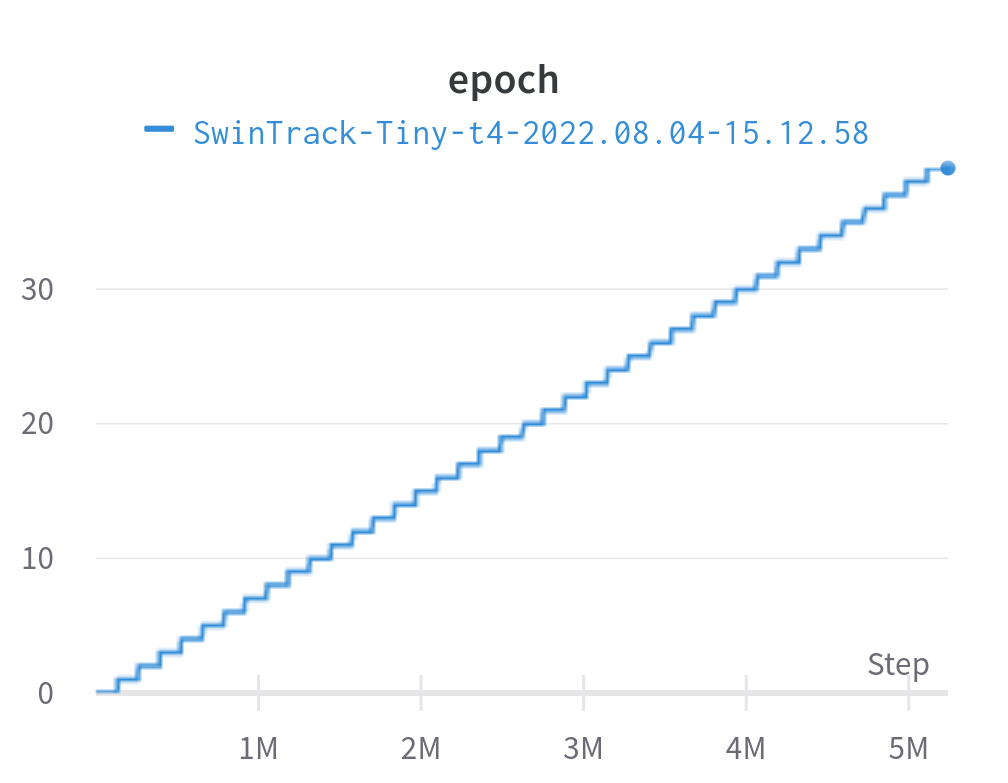
\includegraphics[width=0.7\textwidth]{charts/Section-2-Panel-6-m8q6253z0}}
 	\caption{
 		\textRL{رقم الـ}
 		\textLR{epoch}
 		\textRL{كتابع لرقم  عينة التدريب}}
 	\label{chart:epoch1}
 \end{figure}
  \begin{figure}[H]
 	\centerline{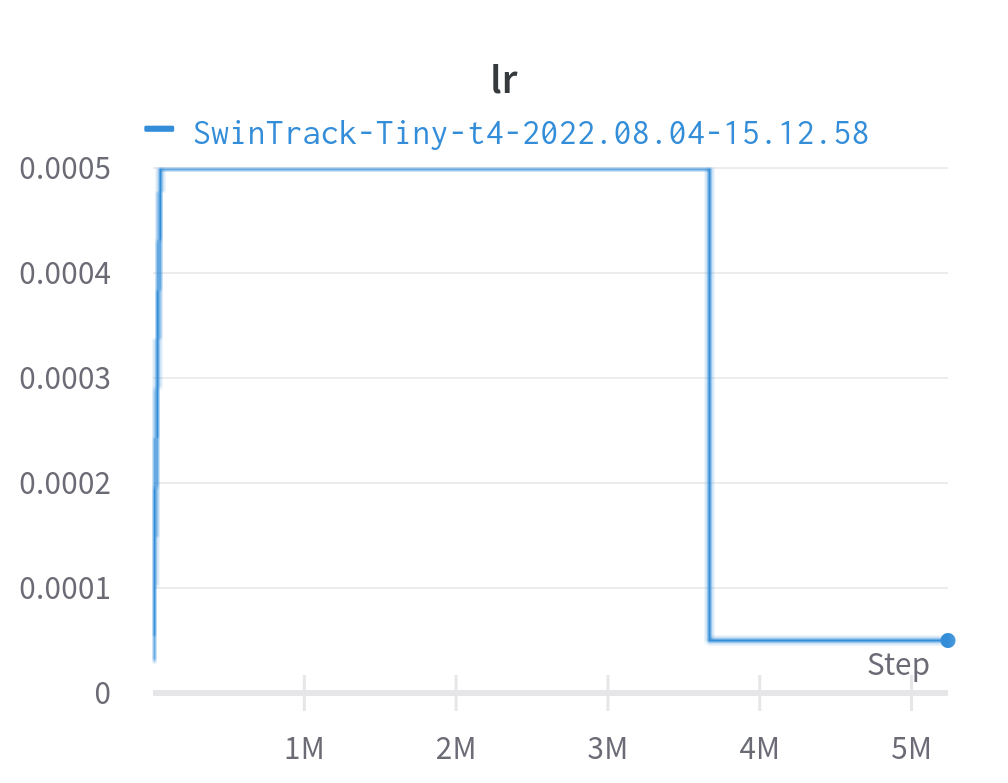
\includegraphics[width=0.7\textwidth]{charts/Section-2-Panel-12-bzoemlec5}}
 	\caption{
 		\textRL{معدل التدريب كتابع لرقم  عينة التدريب}}
 	\label{chart:lr1}
 \end{figure}

\begin{figure}[H]
	\centerline{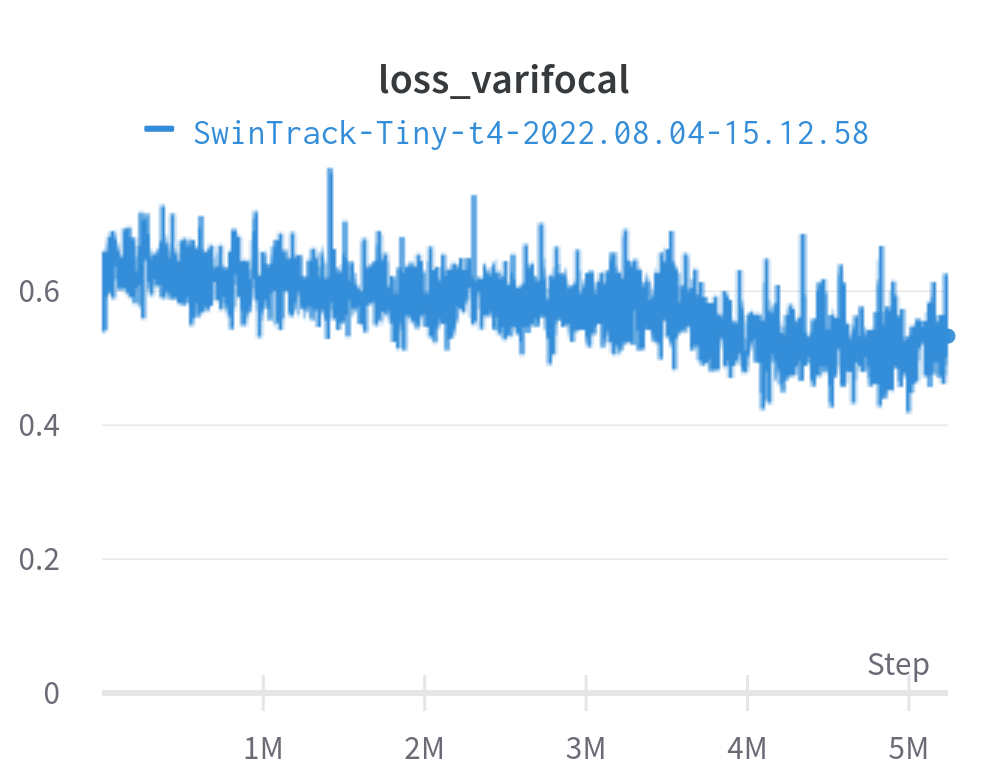
\includegraphics[width=0.7\textwidth]{charts/Section-2-Panel-9-8yjlirrqx}}
	\caption{
		\textRL{تابع خطأ شبكة التصنيف أثناء التدريب}
	}
	\label{chart:loss_varifocal1}
\end{figure}

\begin{figure}[H]
	\centerline{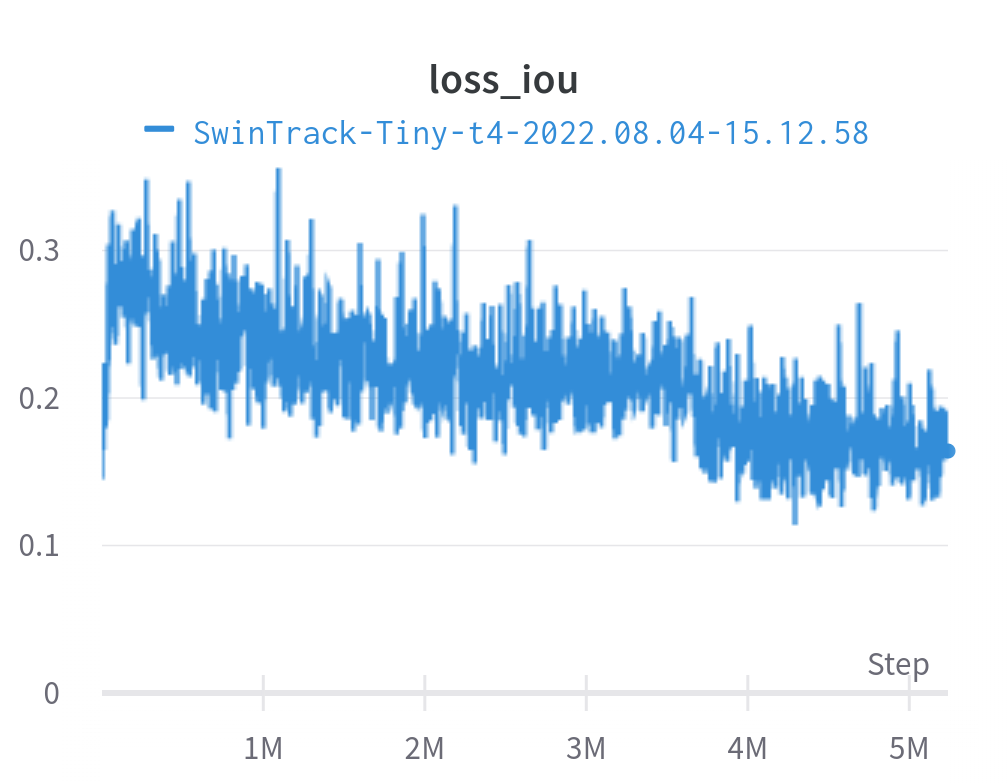
\includegraphics[width=0.7\textwidth]{charts/Section-2-Panel-13-ffs6mrffa}}
	\caption{
		\textRL{تابع خطأ شبكة الـ}
		\textLR{regression}
		\textRL{أثناء التدريب}
	}
	\label{chart:loss_iou1}
\end{figure}

\begin{figure}[H]
	\centerline{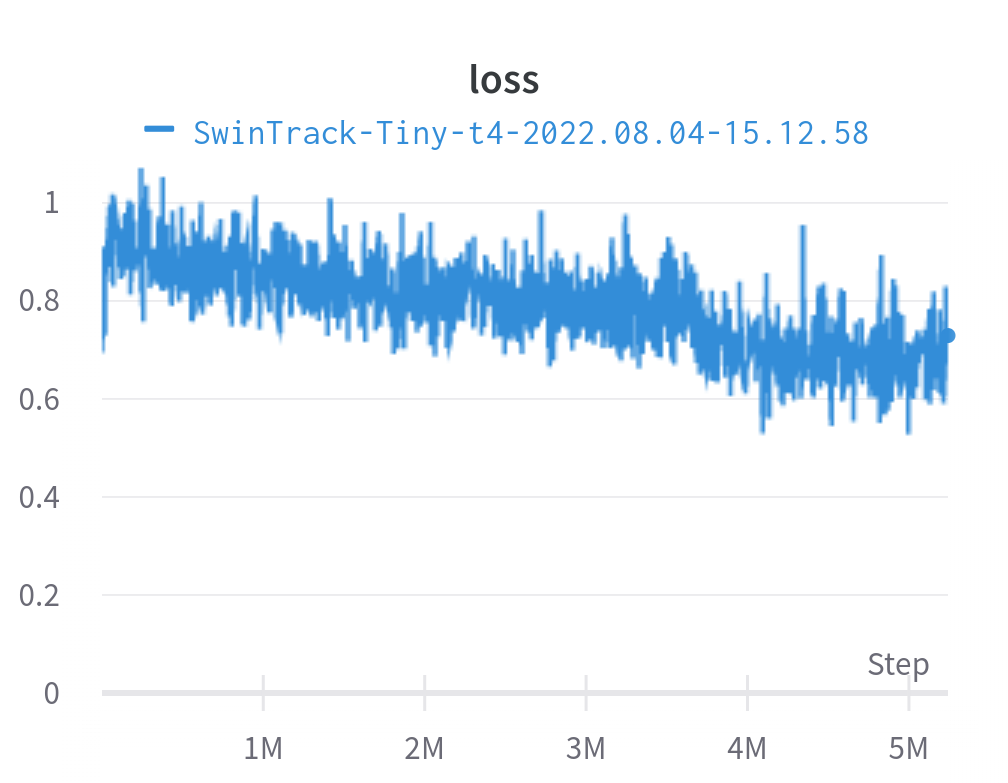
\includegraphics[width=0.7\textwidth]{charts/Section-2-Panel-11-jg4qpu2ty}}
	\caption{
		\textRL{تابع الخطأ الكلي أثناء التدريب}
	}
	\label{chart:loss1}
\end{figure}
\subsubsection{ نتائج التجربة الأولى على مجموعة الـ
\textLR{validation}}
يتم اختبار النموذج على مجموعة الـ
\textLR{validation}
بعد كل 
\textLR{epoch}
وذلك أثناء عملية التدريب.
تبين الأشكال
\ref{chart:val_loss_varifocal},\ref{chart:val_loss_iou},\ref{chart:val_loss}
منحنيات الخطأ لشبكتي التصنيف والـ
\textLR{regression}،
ومنحني الخطأ الكلي.
وكما في منحنيات وسطي الخطأ أثناء التدريب، فإن وسطي خطأ النموذج على معطيات الـ
\textLR{validation} 
في تناقص بعد كل 
\textLR{epoch}.
\begin{figure}[H]
	\centerline{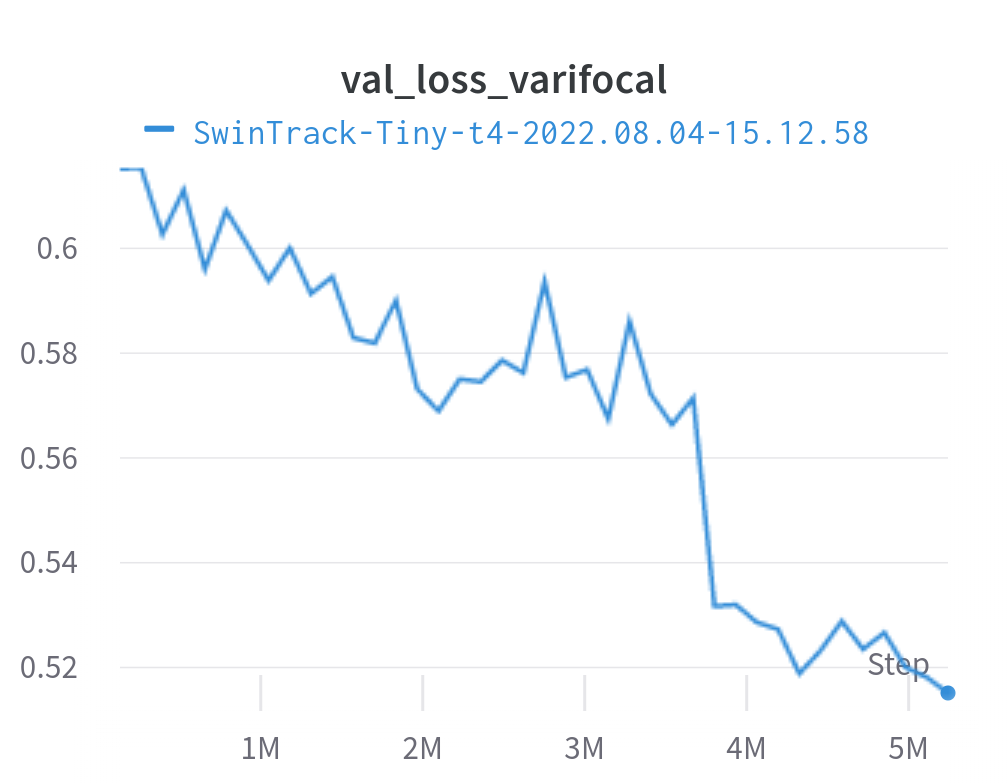
\includegraphics[width=0.7\textwidth]{charts/Section-2-Panel-1-5x2brafi7}}
	\caption{
		\textRL{خطأ شبكة التصنيف على مجموعة الـ}
		\textLR{validation}
	}
	\label{chart:val_loss_varifocal}
\end{figure}

\begin{figure}[H]
	\centerline{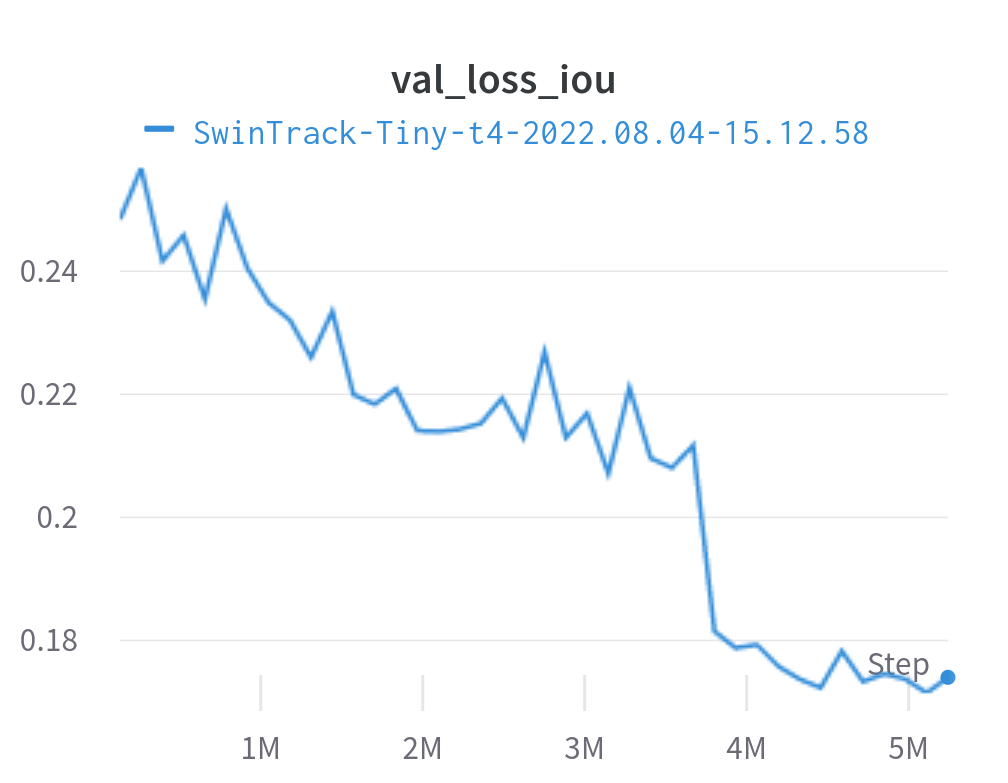
\includegraphics[width=0.7\textwidth]{charts/Section-2-Panel-2-owiohngs7}}
	\caption{
		\textRL{تابع خطأ شبكة الـ}
		\textLR{regression}
		\textRL{على مجموعة الـ}
		\textLR{validation}
	}
	\label{chart:val_loss_iou}
\end{figure}

\begin{figure}[H]
	\centerline{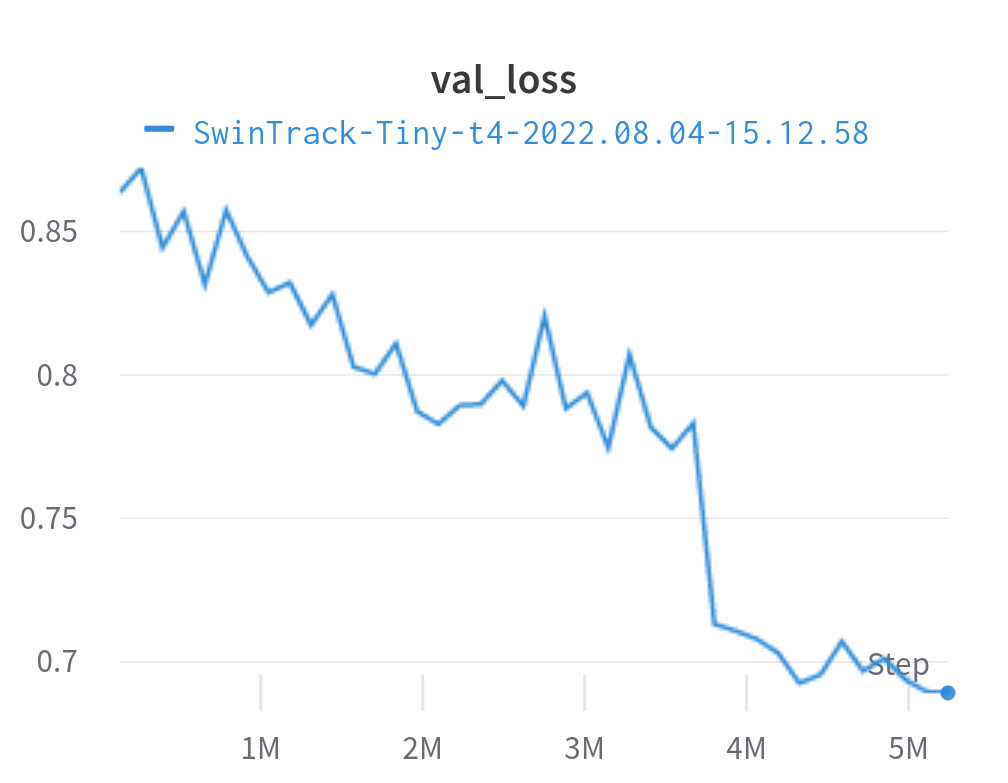
\includegraphics[width=0.7\textwidth]{charts/Section-2-Panel-0-jvrhhrv9d}}
	\caption{
		\textRL{تابع الخطأ الكلي على مجموعة الـ}
		\textLR{validation}
	}
	\label{chart:val_loss}
\end{figure}

%\subsubsection{أداء النظام أثناء التجربة الأولى}
%\selectlanguage{english}
%\begin{figure}[H]
%	\minipage{0.49\textwidth}
%	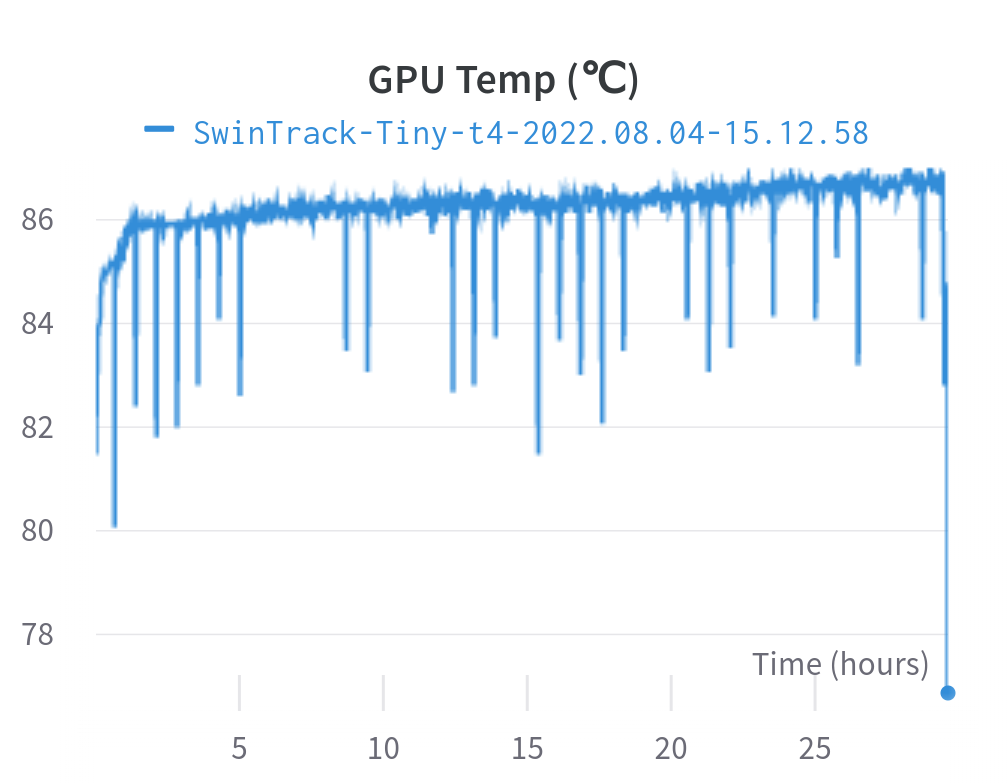
\includegraphics[width=0.7\linewidth]{charts/Section-4-Panel-10-ez7r8q2s1}
%	\caption{\textRL{أثناء التدريب}
%		GPU
%		\textRL{درجة حرارة الـ}}
%	\endminipage\hfill
%	\minipage{0.49\textwidth}
%	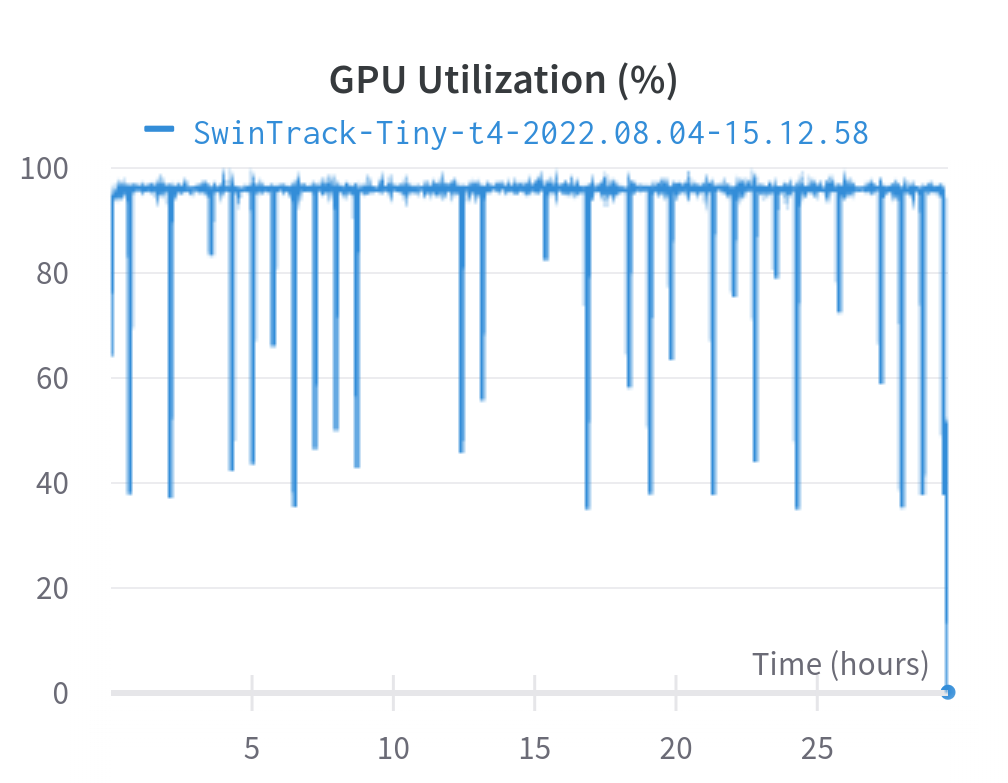
\includegraphics[width=0.7\linewidth]{charts/Section-4-Panel-11-7ugto7ti8}
%	\caption{
%		\textRL{أثناء التدريب}
%		GPU
%		\textRL{نسبة استخدم الـ}}
%	\endminipage
%\end{figure}
%\begin{figure}[H]
%	\minipage{0.49\textwidth}
%	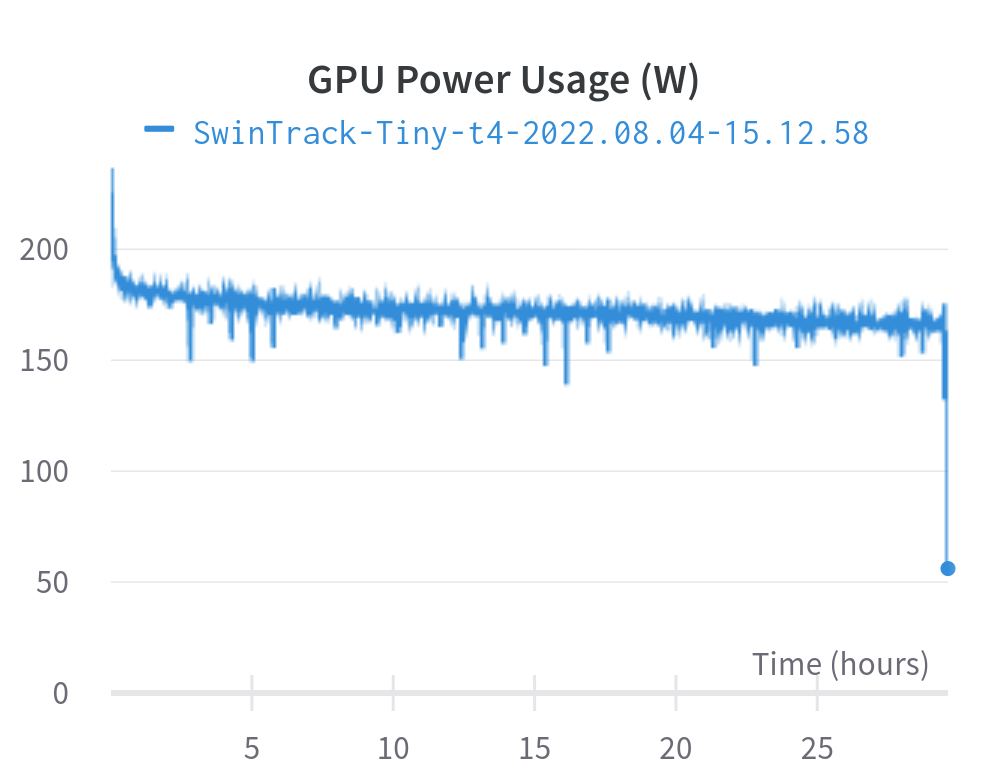
\includegraphics[width=0.7\linewidth]{charts/Section-4-Panel-6-0i8v5s4ys}
%	\caption{GPU
%		\textRL{نسبة استهلاك الطاقة للـ}}
%	\endminipage\hfill
%\end{figure}
%\selectlanguage{arabic}
\subsection{التجربة الثانية}
تم تجريب كتلة انتباه تقاطعي بثمانية رؤوس
$h = 8$.
مع استخدام أوزان النموذج المدرب في التجربة الأولى كأوزان ابتدائية، وأثناء التدريب تم تجميد الأوزان ما عدا أوزان كتلة الانتباه.
تم التدريب عن طريق وحدة معالجة الرسومات 
\textLR{GPU NVIDIA GeForce 3060 Ti}
واختيار 
\textLR{Epoches = 9 , Batch size=1}.
\subsection{عرض ومناقشة النتائح}
سنعرض في هذه الفقرة نتائج اختبار النموذج من أجل التجربتين السابقتين على مجموعة الـ
\textLR{validation}،
وعلى مجموعة الاختبار 
\textLR{testing}.
وبما أننا لا نملك القيم الحقيقية لمجموعة الاختبار، وبما أن مجموعة الاختبار لا تتقاطع مع مجموعتي التدريب والـ 
\textLR{validation}
من حيث صنف الغرض، فسيكون تقييم النموذج على مجموعة الاختبار هو الأكثر أهمية، لأنه يعبر عن قدرة النموذج على التعميم.
\newline
يوضح الجدول
\ref{table:my_model_compare_val}
نتائج الاختبار على مجموعة الـ
\textLR{validation}
الخاصة بـ
\textLR{GOT-10k}،
وذلك من أجل الخوارزمية الأساسية 
\textLR{SwinTrack-Tiny\cite{swinTrack}}،
ومن أجل التجربتين الموضحتين سابقاَ. وبما أننا أضفنا تابع انتباه بأربع رؤوس مع إضافة معلومات زمانية فرمزنا للنموذج في التجربة الأولى بـ
\textLR{SwinTrack-t4}.
ولنموذج التجربة الثانية بـ 
\textLR{SwinTrack-t8}،
كوننا استخدمنا تابع انتباه بثمانية
$8$
رؤوس.
\newline
أما الجدول 
\ref{table:my_model_compare_test}
فيوضح نتائج اختبار الخوارزميات السابقة على مجموعة الاختبار 
\textLR{testing}.
%\selectlanguage{english}
\begin{table}[H]
	\centering
	\begin{tabular}{c |c| c |c} 
		\hline
		& \textLR{SwinTrack-Tiny} & \textLR{SwinTrack-t4} & \textLR{SwinTrack-t8}\\[0.5ex] 
		\hline\hline
		$AO$ & $69.6$& $70.4$&$69.8$\\
		$SR_{0.50}$ &$79.5$&$81.1$&$80.3$\\ 
		$SR_{0.75}$ &$64.8$&$63.2$&$63.6$\\
		$Hz$ &&&\\[1ex] 
		\hline
	\end{tabular}
	\caption{\textRL{نتائج اختبار  النماذج من أجل مجموعة}
	\textLR{testing-GOT-10k}}
	\label{table:my_model_compare_test}
\end{table}

\begin{table}[H]
	\centering
	\begin{tabular}{c |c |c| c} 
		\hline
		 & \textLR{SwinTrack-Tiny} & \textLR{SwinTrack-t4} & \textLR{SwinTrack-t8}\\[0.5ex] 
		\hline\hline
		\textLR{update interval} & &$10 $&$30$\\
		\textLR{iou threshold} &&&$0.8$\\ 
		\textLR{Success Score} &$81.6$&$79.2$&$79.8$\\
		\textLR{Precision Score} &$75.1$&$71.2$&$72.3$\\
		\textLR{Normalized Precision Score} &$91.7$&$89.7$&$90.2$\\
		\textLR{Average Overlap} &$83.2$&$80.7$&$81.3$\\
		$SR_{0.5}$&$93.2$&$90.8$&$91.6$\\
		$SR_{0.75}$&$81.8$&$78.1$&$80$\\
		$FPS$&$88$&$72$&$88$\\
		\textLR{params(M)}&$22.7$&$23.3$&$23.3$\\[1ex] 
		\hline
	\end{tabular}
	\caption{\textRL{نتائج اختبار  النماذج من أجل مجموعة}
	\textLR{validation-GOT-10k}}
	\label{table:my_model_compare_val}
\end{table}


%report
\begin{table}[H]
	\centering
	\begin{tabular}{c |c |c| c} 
		\hline
		& \textLR{SwinTrack-Tiny} & \textLR{SwinTrack-t4} & \textLR{SwinTrack-t8}\\[0.5ex] 
		\hline\hline
		\textLR{update interval} & &$10 $&$30$\\
		\textLR{iou threshold} &&&$0.8$\\ 
		\textLR{Average Overlap} &$83.2$&$80.7$&$81.3$\\
		$SR_{0.5}$&$93.2$&$90.8$&$91.6$\\
		$SR_{0.75}$&$81.8$&$78.1$&$80$\\
		$FPS$&$88$&$72$&$88$\\
		\textLR{params(M)}&$22.7$&$23.3$&$23.3$\\[1ex] 
		\hline
	\end{tabular}
	\caption{\textRL{نتائج اختبار  النماذج من أجل مجموعة}
		\textLR{validation-GOT-10k}}
	\label{table:my_model_compare_val}
\end{table}


\selectlanguage{arabic}

\begin{table}[H]
	\centering
	\begin{tabular}{c |c| c |c} 
		\hline
		\textRL{النموذج}& $AO$ & $SR_{0.50}$ & $SR_{0.75}$\\[0.5ex] 
		\hline\hline
		\textLR{Ours-t4}&\textcolor{red}{$70.4$}&\textcolor{red}{$81.1$}&$63.2$\\
		\textLR{Ours-t8}&\textcolor{blue}{$69.8$}&\textcolor{blue}{$80.3$}&\textcolor{blue}{$63.6$}\\
		\textLR{SwinTrack-B}&$69.4$&$78$&\textcolor{red}{$64.3$}\\[1ex] 
		\textLR{SLT-TransT}&$67.5$&$76.8$&$60.3$\\
		\textLR{TREG}&$66.8$&$77.8$&$57.2$\\
		\textLR{Siam R-CNN}&$64.9$&$72.8$&\\
		\textLR{STMTrack}&$64.2$&$73.7$&$57.5$\\
		\textLR{Ocean}&$61.1$&$72.1$&\\
		\textLR{DiMP}&$61.1$&$71.7$&\\
		\textLR{SiamFC++}&$61.0$&$74.2$&\\
		\textLR{ATOM}&$55.6$&$63.4$&\\[1ex]
		\hline
	\end{tabular}
	\caption{\textRL{مقارنة بين عدة خوارزميات ملاحقة من أجل مجموعة}
	\textLR{testing-GOT-10k}}
	\label{table:my_model_compare_test}
\end{table}



%report
\begin{table}[H]
	\centering
	\begin{tabular}{c |c| c |c|c} 
		\hline
		\textRL{النموذج}& $AO$ & $SR_{0.50}$ & $SR_{0.75}$& \textLR{year}\\[0.5ex] 
		\hline\hline
		\textLR{Ours-t4}&\textcolor{red}{$70.4$}&\textcolor{red}{$81.1$}&$63.2$&$2022$\\
		\textLR{Ours-t8}&\textcolor{blue}{$69.8$}&\textcolor{blue}{$80.3$}&\textcolor{blue}{$63.6$}&$2022$\\
		\textLR{SwinTrack-B}&$69.4$&$78$&\textcolor{red}{$64.3$}&$2021$\\[1ex] 
		\textLR{SLT-TransT}&$67.5$&$76.8$&$60.3$&$2022$\\
		\textLR{TREG}&$66.8$&$77.8$&$57.2$&$2021$\\
		\textLR{Siam R-CNN}&$64.9$&$72.8$&&$2019$\\
		\textLR{STMTrack}&$64.2$&$73.7$&$57.5$&$2021$\\
		\textLR{Ocean}&$61.1$&$72.1$&&$2020$\\
		\textLR{DiMP}&$61.1$&$71.7$&&$2019$\\
		\textLR{SiamFC++}&$61.0$&$74.2$&&$2019$\\
		\textLR{ATOM}&$55.6$&$63.4$&&$2018$\\[1ex]
		\hline
	\end{tabular}
	\caption{\textRL{مقارنة بين عدة خوارزميات ملاحقة من أجل مجموعة}
		\textLR{testing-GOT-10k}}
	\label{table:my_model_compare_test}
\end{table}
نلاحظ من الجدول 
\ref{table:my_model_compare_val}
بمقارنة الخوارزميات السابقة من ناحية السرعة في السطر المقابل لـ 
\textLR{FPS frame by second}،
بأن كتلة الانتباه التي أضفناها مع تحديث الـ
\textLR{template}
كل 
$30$
إطار لم تؤثر على السرعة من أجل $4$ رؤوس، بينما التحديث كل 
$10$
إطارات قد خفض الزمن بمقدار 
$8FPS$
عند الاختبار من أجل
$8$
رؤوس.
ونلاحظ أيضاً أن الأداء لم يتحسن بالنسبة للاختبار على معطيات الـ
\textLR{validation}.
\newline
لكن بالمقابل 
بمقارنة الخوارزميات على مجموعة الاختبار
عن طريق المخدم الخاص بـ
\textLR{GOT-10k}،
وكما يوضحه الجدول 
\ref{table:my_model_compare_test}،
% عند اختبارها على معطيات الـ
%\textLR{testing}
%
فقد تحسن الأداء في كل من التجربتين. في التجربة الأولى
\textLR{SwinTrack-t4}
 فقد تحسنت نسبة
$AO$
بمقدار
$0.8\%$،
و
$1.6\%$
بالنسبة للمقدار
$SR_{0.5}$.
نفسر اختلاف النتائج بالنسبة لمجموعتي الاختبار والـ
\textLR{validation}،
%نفسر ذلك بأن مجموعة الـ
%\textLR{validation}
بأن مجموعة التدريب ومجموعة الـ
\textLR{validation}
تتقاطع من ناحية صنف الغرض والحركة كما ذكرنا في الفقرة
\ref{section:got10k}،
لكنها لاتتقاطع مع معطيات الاختبار.
بالإضافة إلى أن النموذج الأساسي تم تدريبه من أجل 
$Epoches = 300$
بينما نموذج اختبارنا الأول من أجل 
$Epoches = 40$،
ونموذج الاختبار الثاني من أجل 
$Epoches = 9$ 
فقط. وهذا ما يفسر 
\textLR{underfitting}
بالنسبة لمجموعة التدريب والتي مجموعة الـ
\textLR{validation}
جزء منها.
وبنفس الوقت فإن التدريب من أجل 
$epoches$
قليلة وتجميد أوزان النموذج الأساسي وتعديل أوزان كتلة الانتباه فقط، جنب النموذج المعدل الـ
\textLR{overfitting}
وهذا ما يفسر تحسن الأداء بالنسبة لمعطيات الـ
\textLR{testing}،
والتي تختلف عن معطيات التدريب والـ
\textLR{validation}.
\newline
بالنسبة للتجربة الثانية
\textLR{SwinTrack-t8}
 فإن تحسن الأداء كان بنسبة 
$0.2\%$
بالنسبة للـ
$AO$،
وبنسبة 
$0.6\%$
بالنسبة لـ
$SR_{0.5}$.
هذا التحسن الطفيف في الأداء يمكن أن نفسره بأن النموذج لم يدرب بشكل كافي، إذ تم تدريبه على 
\textLR{9 epoches}
فقط،
وذلك بسبب مشاكل تقنية في وحدة معالجة الرسومات 
\textLR{GPU NVIDIA GeForce 2080 Ti}،
لذلك لم نتمكن من تدريب النموذج الثاني عليها.
\newline
من المتوقع أن يتحسن الأداء بشكل أكبر إذا تم تدريب النموذج على عدد أكبر من الـ
$epoches$.
\newline
في كلا التجربتين نلاحظ تراجع قيمة 
$SR_{0.75}$
بمقدار 
$1.6\%$
للنموذج الأول، وبمقدار 
$1.2$
للنموذج الثاني، هذا يعني أن دقة الملاحقة أقل من النموذج الأساسي ولكن عدد الإطارات التي تتم ملاحقتها أكبر، أي أن تحديث صورة الهدف ودمجه مع الصور الابتدائية بالطريقة التي اختبرناها قد جعل الملاحق أكثر صلادة ولكن أقل دقة.
\newline
يبين الجدول 
\ref{table:many_model_compare_test}
مقارنة بين النماذج المتعلقة باختباراتنا في البحث  مع خوارزميات الملاحقة الحديثة التي تتصدر أفضل أداء بالنسبة لمجموعة المعطيات 
\textLR{GOT-10k\cite{got10k}}،
وذلك عند البدء في البحث في عام
$2022$.
\newline
أما بالنسبة لمنحنيات التقييم فيوضح الشكلان
\ref{fig:successCurve}
و
\ref{fig:precision}
منحنيات النجاح والدقة بالنسبة للنماذج الثلاثة المذكور سابقاَ، وذلك من أجل مجموعة الـ
\textLR{validation}،
حيث النموذج الأصلي 
\textLR{SwinTrack-Tiny}
باللون الأزرق، و
\textLR{SwinTrack-t4}
باللون الأخضر، أما
\textLR{SwinTrack-t8}
باللون البرتقالي.
وكما ذكرنا سابقاً فإن أداء النماذج المعدلة لم يتحسن بالنسبة لمجموعة الـ
\textLR{validation}،
وهذا مايفسر تواجد منحنيات النموذجين المعدلين
أسفل النموذج الأصلي
\textLR{SwinTrack-Tiny}
\begin{figure}[H]
	\centerline{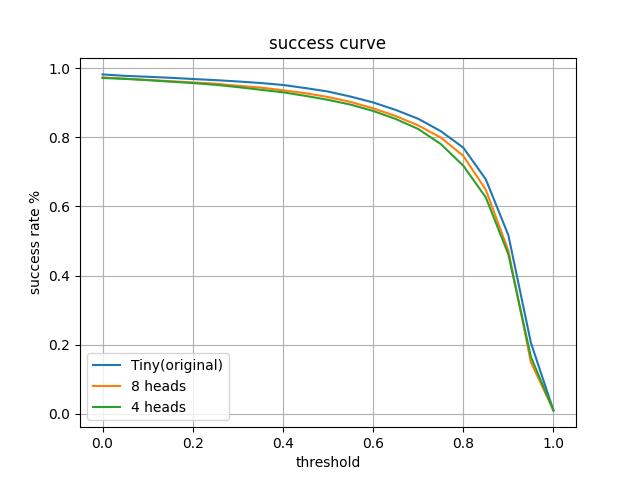
\includegraphics[width=\textwidth]{charts/successCurve}}
	\caption{\textRL{
					منحني النجاح للنماذج الثلاثة، اللون الأزرق هو النموذج الأصلي،
		}}
	\label{fig:successCurve}
\end{figure}
\vspace{-13.0mm}
\textRL{
			 اللون الأخضر هو التجربة الأولى بكتلة انتباه
			بـ 
			$4$ 
			رؤوس، واللون البرتقالي هو التجربة الثانية بـ
			$8$
			رؤوس
}


\begin{figure}[H]
	\centerline{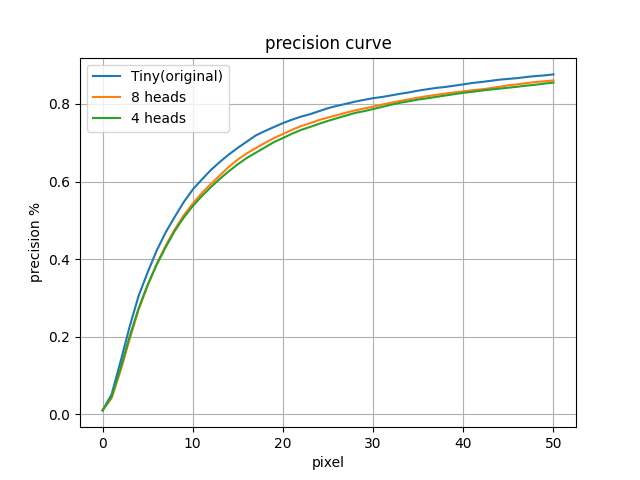
\includegraphics[width=\textwidth]{charts/precision curve}}
	\caption{\textRL{منحني الدقة للنماذج الثلاثة}}
	\label{fig:precision}
\end{figure}

\subsubsection{اختبارت الخوارزميات على  الفيديو}
اختبرنا الخوارزميات السابقة على عدة فيديوهات من مجموعة الـ 
\textLR{validation}، 
وأظهرنا نتائج الملاحقة في الصور التالية، بحيث يقابل كل لون من ألوان المستطيلات إلى خوارزمية وفق مايلي:
%ألوان النماذج كمايلي
\begin{itemize}
	\item 	القيم الحقيقة باللون الأخضر
	\item
	النموذج الأصلي 
	\textLR{SwinTrack-Tiny}
	باللون الأصفر
	\item
	نموذج التجربة الأولى
	\textLR{SwinTrack-t4}
	باللون الزهري
	\item
	نموذج التجربة الثانية
	\textLR{SwinTrack-t8}
	باللون السماوي
\end{itemize}

في الشكل
\ref{fig:video_success_1}
مثال عن نجاح النماذج في الملاحقة، ولكن النموذج الأصلي بدقة أقل من النموذجين المعدلين، وذلك بسبب وجود أغراض مشابهة للغرض الملاحَق.
\begin{figure}[H]
	\centerline{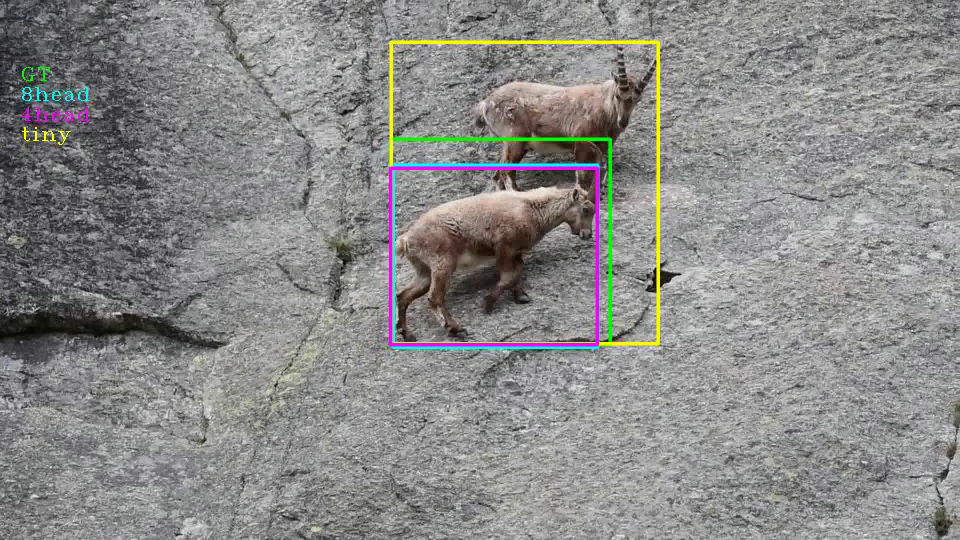
\includegraphics[width=\textwidth]{images/results/success/project_52}}
	\caption{\textRL{مثال عن الملاحقة مع وجود أغراض مشابهة}}
	\label{fig:video_success_1}
\end{figure}
أيضاً بالنسبة للشكل
\ref{fig:video_success_2}
فإن النموذج الأصلي يفشل في الملاحقة، بينما النموذج المعدل حسن من الأداء في هذه الحالة.
\begin{figure}[H]
	\centerline{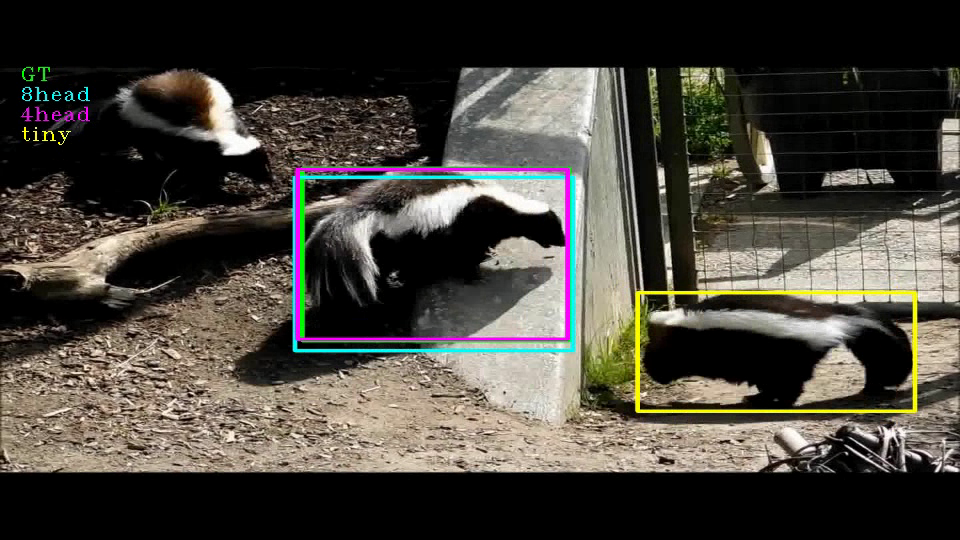
\includegraphics[width=\textwidth]{images/results/success/project_161}}
	\caption{\textRL{مثال عن الملاحقة مع وجود أغراض مشابهة}}
	\label{fig:video_success_2}
\end{figure}
في الشكل 
\ref{fig:video_success_3_initial}
نتيجة الملاحقة في بداية الفيديو، وعندما يتغير شكل الغرض بشكل كبير كما في الشكل 
\ref{fig:video_success_3}،
فإن النموذج الأصلي لا يستطيع أن يحدد مكان الغرض بدقة النموذجين المعدلين، وذلك كون التعديل المضاف يأخذ بعين الإعتبار التغيرات التي تطرأ على شكل الغرض، ويدخلها إلى النموذج من جديد.
\begin{figure}[H]
	\centerline{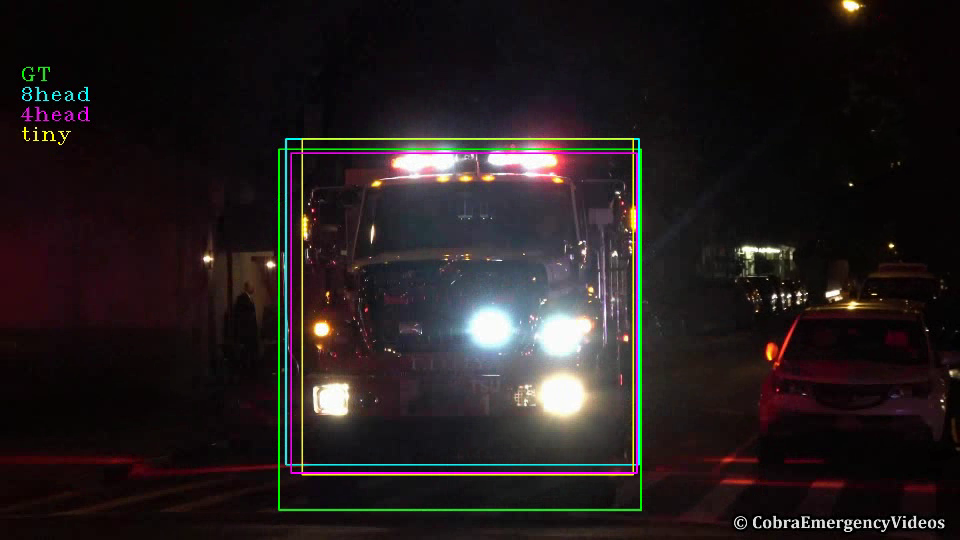
\includegraphics[width=\textwidth]{images/results/success/project_1802}}
	\caption{\textRL{مثال عن الملاحقة مع تغير كبير في شكل الغرض}}
	\label{fig:video_success_3_initial}
\end{figure}

\begin{figure}[H]
	\centerline{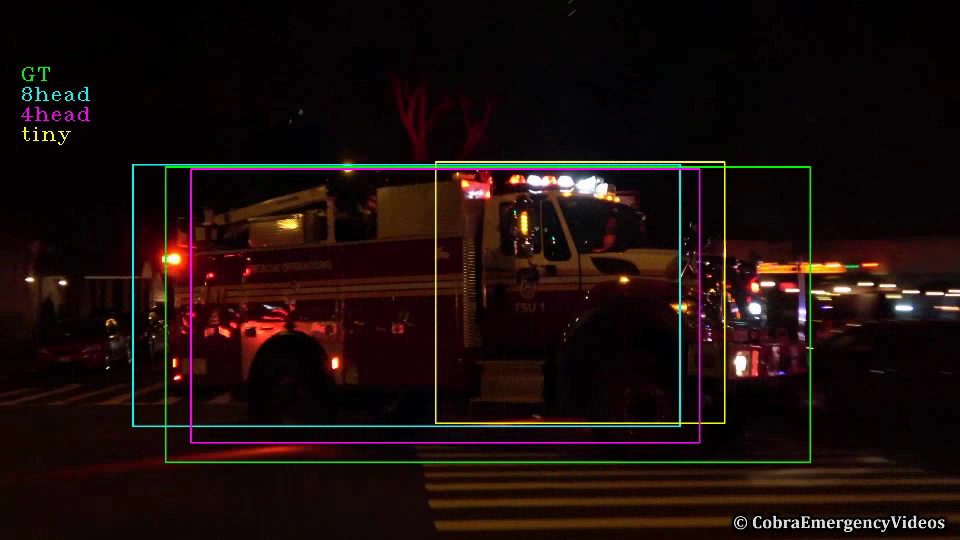
\includegraphics[width=\textwidth]{images/results/success/project_180}}
	\caption{\textRL{مثال عن الملاحقة مع تغير كبير في شكل الغرض}}
	\label{fig:video_success_3}
\end{figure}
أما في الشكل
	\ref{fig:video_fail_1_initial}
	فيكون المطلوب ملاحقة أغراض صغيرة، ووجود أغراض مشابهة بجوار الغرض المطلوب.
	هنا نرى في الشكل 
	\ref{fig:video_fail_1}
	فشل النموذجين المعدلين بينما ينجح النموذج الأصلي في هذه الحالة.
\begin{figure}[H]
	\centerline{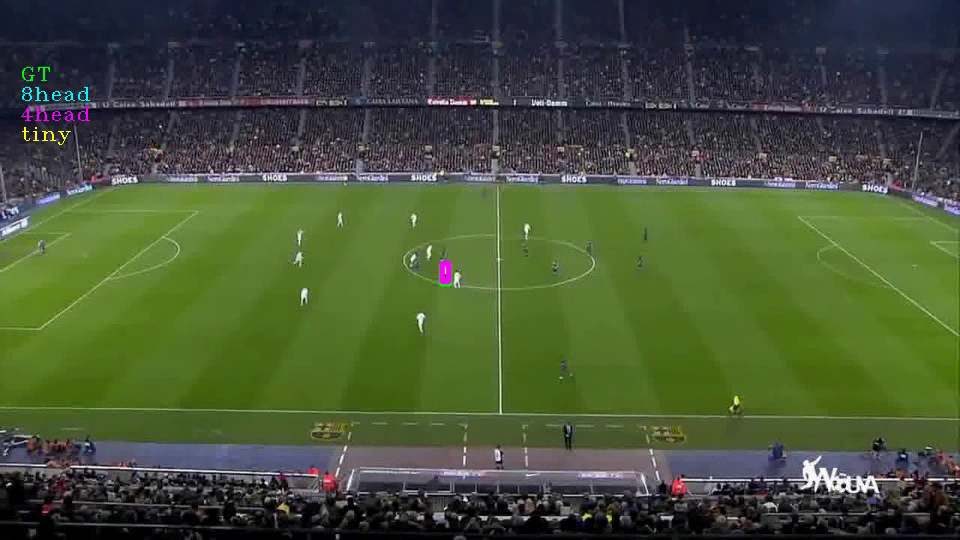
\includegraphics[width=\textwidth]{images/results/failed/project_175.avi}}
	\caption{\textRL{ 
			مثال عن ملاحقة أغراض صغيرة - بداية عملية الملاحقة
	}}
	\label{fig:video_fail_1_initial}
\end{figure}

\begin{figure}[H]
	\centerline{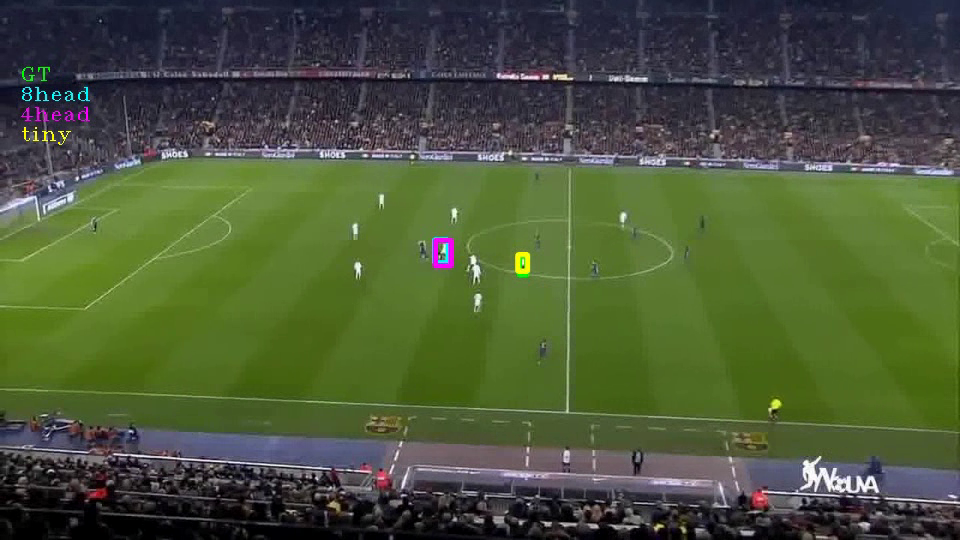
\includegraphics[width=\textwidth]{images/results/failed/project_175.avi1}}
	\caption{\textRL{
			مثال عن ملاحقة أغراض صغيرة - أثناء عملية الملاحقة
	}}
	\label{fig:video_fail_1}
\end{figure}	
	وأيضا فيما يتعلق بالشكلين
	\ref{fig:video_fail_2_initial}
		و
	\ref{fig:video_fail_2}.
	نستنتج من الفيديوهات السابقة أن التعديل قد حسن من الأداء من أجل الأغراض التي يتغير مظهرها بشكل كبير، لكن ليس من أجل الأغراض الصغيرة أو في حالة وجود أغراض مشابهة للغرض المطلوب ملاحقته.
	هنا يمكن تفسير ذلك بأن النموذجين المعدلين مدربان على أخذ تغير مظهر الغرض بعين الاعتبار، وبالتالي عند وجود أغراض مشابهة فإنه لايستطيع التمييز بينها وبين الغرض المطلوب ملاحقته في أثناء تغير مظهره.
\begin{figure}[H]
	\centerline{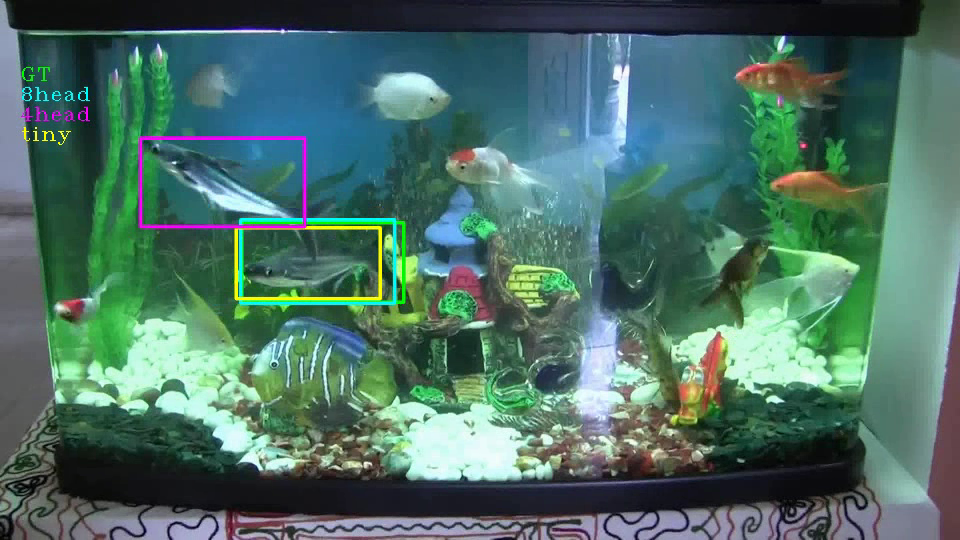
\includegraphics[width=\textwidth]{images/results/failed/project_129.avi2}}
	\caption{\textRL{مثال عن الملاحقة مع وجود أغراض مشابهة}}
	\label{fig:video_fail_2_initial}
\end{figure}

\begin{figure}[H]
	\centerline{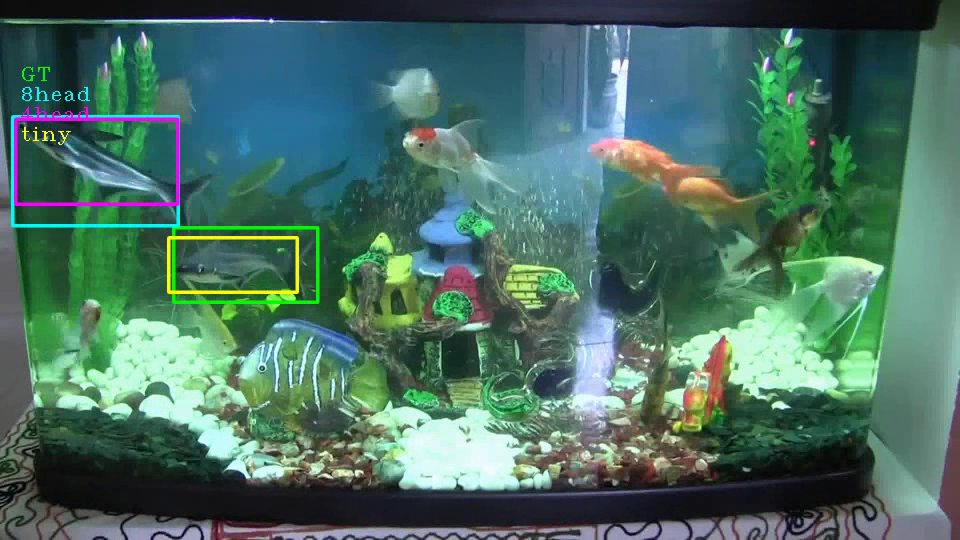
\includegraphics[width=\textwidth]{images/results/failed/project_129.avi3}}
	\caption{\textRL{مثال عن الملاحقة مع وجود أغراض مشابهة}}
	\label{fig:video_fail_2}
\end{figure}
